%Created with command:
%"/home/josh/Teaching/trunk/Utilities/makeexam" "Homework 2 - CMOS and TTL Circuits" "Attempt the following problems.  Please show all of your work.  You may work with others however make sure that all work you submit is yours." "../CMOSCircuits/Assessments/cmos_AND_gate_analysis.tex" "../CMOSCircuits/Assessments/cmos_nand_nor_conversion_to_logic_diagram.tex" "../CMOSCircuits/Assessments/dc_noise_margin.tex" "../CMOSCircuits/Assessments/wakerly_3_61.tex" "../TTLCircuits/Assessments/ttl_buffer.tex"
\documentclass{article}
\usepackage[T1]{fontenc}
\usepackage{arev}
\usepackage{longtable}
\usepackage[hmargin=2cm,vmargin=2cm]{geometry}
\usepackage{graphicx}
\setlength{\parindent}{0pt}
\title{Homework 2 - CMOS and TTL Circuits}
\date{}
\begin{document}
\maketitle
Attempt the following problems.  Please show all of your work.  You may work with others, however make sure that all work you submit is yours. (16 points total)
\begin{longtable}[l]{rp{17cm}}
%file: ../CMOSCircuits/Assessments/cmos_AND_gate_analysis.tex
1.&\begin{minipage}[t]{\linewidth}(4 pt) Determine the function table for the following CMOS logic gate.  Is this a standard gate?  If so, which gate is it? \\ \\
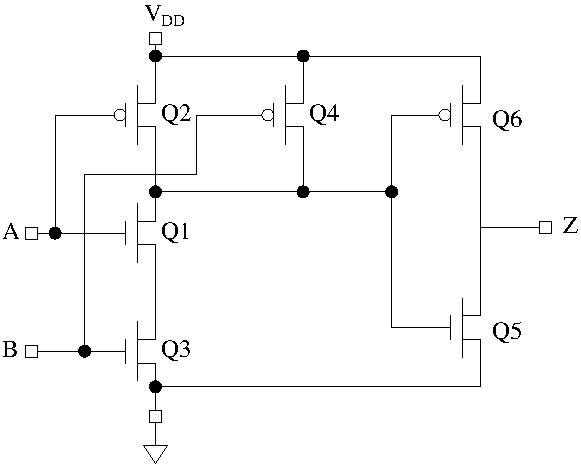
\includegraphics{../CMOSCircuits/Assessments/CMOSANDGate}\\

\vspace{8cm
}
\end{minipage}\\
\medskip
%file: ../CMOSCircuits/Assessments/cmos_nand_nor_conversion_to_logic_diagram.tex
2.&\begin{minipage}[t]{\linewidth}(2 pt) Convert the following CMOS circuit to a logic diagram.\\ \\
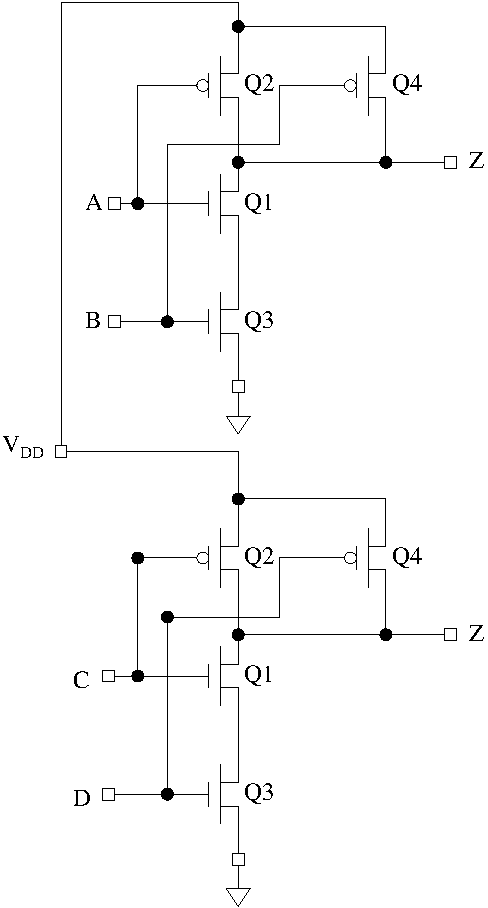
\includegraphics{../CMOSCircuits/Assessments/CMOSNANDNOR}

\vspace{8cm
}
\end{minipage}\\
\medskip
%file: ../CMOSCircuits/Assessments/dc_noise_margin.tex
3.&\begin{minipage}[t]{\linewidth}(2 pt) Given the following information from a data sheet, compute the HIGH and LOW state DC noise margins.\\ \\
$\textrm{V}_{\textrm{OHmin}} = 4.9 \textrm{V}$\\
$\textrm{V}_{\textrm{IHmin}} = 3.5 \textrm{V}$\\
$\textrm{V}_{\textrm{ILmax}} = 1.5 \textrm{V}$\\
$\textrm{V}_{\textrm{OLmax}} = 0.2 \textrm{V}$\\

\vspace{4cm
}
\end{minipage}\\
\medskip
%file: ../CMOSCircuits/Assessments/wakerly_3_61.tex
4.&\begin{minipage}[t]{\linewidth}(4 pt) Do problem 3.61 in the text.\\ \\

\vspace{12cm
}
\end{minipage}\\
\medskip
%file: ../TTLCircuits/Assessments/ttl_buffer.tex
5.&\begin{minipage}[t]{\linewidth}(4 pt) Use bipolar junction transistors to design a one input TLL buffer circuit.\\ \\

\vspace{6cm
}
\end{minipage}\\
\medskip
\end{longtable}
\end{document}